\documentclass[12pt,openany,a4paper]{book}

% Font and page layout
\usepackage[T1]{fontenc}
\usepackage[utf8]{inputenc}
\usepackage{lmodern}
\usepackage[margin=2.5cm]{geometry}
\usepackage{setspace}
\usepackage{parskip}
\usepackage{microtype}

% Colour and table formatting
\usepackage{xcolor}
\usepackage{graphicx}
\usepackage{float}
\usepackage{array}
\usepackage{multirow}
\usepackage{makecell}


\setstretch{1.15}
\setlength{\emergencystretch}{3em}

\definecolor{instruc}{RGB}{112,48,160}

%For Maths
\usepackage{amsmath}
\usepackage{amssymb}

% Bibliography
\usepackage[numbers,sort&compress]{natbib}
% Make \doi read its argument verbatim so DOIs containing _ ~ & etc. don't break
\usepackage{url}
\DeclareUrlCommand\doi{\urlstyle{rm}}

% Instructional formatting
\newcommand{\instructionstyle}{%
  \color{instruc}%
  \itshape%
  \fontsize{11pt}{12pt}\selectfont%
}

% For short instructional text, including table entries
\newcommand{\instructiontext}[1]{%
  {\instructionstyle #1}%
}

% For longer instructional blocks
\newenvironment{instructions}
  {\par\begingroup\instructionstyle}
  {\par\endgroup}

% Rotated table headings
\newcommand{\rotatedheading}[1]{%
  \rotatebox[origin=c]{90}{%
    \makebox[4.7cm][l]{#1}%
  }%
}

%%%%%%%%%%%%%%%%%%%%%%%%%%%%%%%%%%%%%%%%%%%%%%%%%%%%%%%%%%%%
%%%%%%%%%%%%%%%%%%%% Start Document %%%%%%%%%%%%%%%%%%%%%%%%
%%%%%%%%%%%%%%%%%%%%%%%%%%%%%%%%%%%%%%%%%%%%%%%%%%%%%%%%%%%%

\begin{document}
\section*{Thesis Plan}
\pagestyle{empty} % No page numbers

\subsection*{Student Details}

Student name: Alex Gu\\
Student number: 48028903\\
Program enrolment: Bachelor of Computer Science (Honours)\\
Course enrolment: REIT4881\\
Number of units: 8\\
Expected workload for your enrolment (hours per week): 20

\subsection*{Supervisor Details}

Primary Supervisor: Ruihong Qiu\\
Other Supervisors (optional): Zi (Helen) Huang\\
Have you met your supervisor this semester (yes/no, online/in person): Yes, in person\\
Do you have a regular meeting scheduled for this semester (weekly/biweekly/other---please specify): Other, meetings scheduled as needed


\subsection*{Thesis plan (thesis draft)}


\subsection*{Use of Generative AI Statement}

\subsubsection*{Have you used AI in your project}
\begin{itemize}
  \item Explore your topic? Yes -- discussed federated learning and privacy concepts with Claude to build understanding
  \item Define your research question? No -- research question was defined through meetings with supervisors
  \item Assist with your literature review? Yes -- used Claude to generate notes, verified against originals
  \item Assist with formatting the answers presented here? Yes -- used Claude for LaTeX troubleshooting and guidance on restructuring proposal material into the thesis template
  \item To generate figures? No -- figures were created manually
  \item To analyse data? No -- no experimental data has been analysed yet; analysis will be performed with my own code
  \item To generate data? No -- all data comes from publicly available Kaggle datasets
  \item To generate text for your thesis? No -- thesis text is my own writing, reused from my project proposal where permitted
  \item Other aspects of your work? Yes -- feedback on writing voice and tone
\end{itemize}

\newpage

%%%%%%%%%%%%%%%%%%%%%%%%%%%%%%%%%%%%%%%%%%%%%%%%%%%%%%%%%%%%%%%%%%%
%%%%%%%%%%%%%%%%%%%% Start Thesis Document %%%%%%%%%%%%%%%%%%%%%%%%
%%%%%%%%%%%%%%%%%%%%%%%%%%%%%%%%%%%%%%%%%%%%%%%%%%%%%%%%%%%%%%%%%%%

\let\origcleardoublepage\cleardoublepage
\let\cleardoublepage\clearpage
\frontmatter
\let\cleardoublepage\origcleardoublepage
% By default, frontmatter has Roman page-numbering (i,ii,...).

\begin{titlepage}
\renewcommand{\baselinestretch}{1.0}
\begin{center}
\vspace*{35mm}
\Huge\bf
		
        \begin{figure}[htpb]
            \centering
            
\includegraphics[width=0.6\linewidth]{UQ_Logo.png}
        \end{figure}
        
        \vspace*{25mm}
        
        Privacy-Preserving Federated Learning\\
        for Distributed Skin Disease Classification\\
\vspace{20mm}
\large\sl
		by\\
		ALEX GU
		\medskip\\
\rm
		School of Electrical Engineering and Computer Science,\\
		The University of Queensland.\\
\vspace{30mm}
		Submitted for the degree of Bachelor of Computer Science (Honours) as part\\
        of the course REIT4881.
		\bigskip\\
\large
		August 2026
\end{center}
\end{titlepage}

\newpage

\newpage

\begin{flushright}
	Alex Gu\\
	alex.gu@student.uq.edu.au
	\medskip
\end{flushright}
\begin{flushleft}
  \medskip
  August 2026\\
  \bigskip\bigskip
  Prof Michael Bruenig\\
  Head of School\\
  School of Electrical Engineering and Computer Science\\
  The University of Queensland\\
  St Lucia, Q 4072\\
  \bigskip\bigskip
  Dear Professor Bruenig,
\end{flushleft}

In accordance with the requirements of the Degree of Bachelor of Computer Science (Honours) in the School of Electrical Engineering and Computer Science, I submit the following thesis entitled\\\\
\centerline{``Privacy-Preserving Federated Learning for Distributed Skin Disease Classification''}\\\\
The thesis was performed under the supervision of Dr Ruihong Qiu. I declare that the work submitted in the thesis is my own, except as acknowledged in the text and footnotes, and that it has not previously been submitted for a degree at the University of Queensland or any other institution.


\begin{flushright}
	Yours sincerely,\\
	\medskip
	\emph{\{Author's Signature\}}\\
	\medskip
	ALEX GU
\end{flushright}

\chapter{Declaration by Author}

This thesis is composed of my original work, and contains no material previously published, written by another person, or generated by artificial intelligence (AI), except where clearly referenced and acknowledged either in the main text or the preliminary pages of this thesis. I have clearly stated the contribution of others to jointly authored works that I have included in my thesis.\\

I have clearly stated the contribution of others to my thesis as a whole, including statistical assistance, survey design, data analysis, significant technical procedures, professional editorial advice, use of AI tools, financial support, and any other original research work used or reported in my thesis. The content of my thesis is the result of work I have carried out since the commencement of my enrollment in the course code indicated on the title page, and does not include a substantial part of work that has been submitted to qualify for the award of any other degree or diploma in any university or other tertiary institution. I have clearly stated which parts of my thesis, if any, have been submitted to qualify for another award.\\

I acknowledge that copyright of all material contained in my thesis resides with the copyright holder(s) of that material. Where appropriate I have obtained copyright permission from the copyright holder to reproduce material in this thesis and have sought permission from co-authors for any jointly authored works included in the thesis.

\chapter{Use of AI Statement}


\emph{I acknowledge the use of generative AI tools in completing this
assessment. Details of which tools were used and how they were used are
provided in the table below, along with appropriate in-text and full
references. I take responsibility for critically evaluating and
integrating the AI generated content, and ensuring it adheres to
academic integrity standards.}

\begin{tabular}{
|c|c|c|c|c|c|c|c|c|c|c|
>{\centering\arraybackslash}p{4.45cm}|
}
\hline

\multirow{2}{*}{%
  \parbox{2.5cm}{%
    \centering
     \textbf{AI model and date}
  }%
}
& \multicolumn{11}{c|}{%
    \textbf{Artificial Intelligence (AI) tool usage}
    (tick all that apply)
  }
\\ \cline{2-12}

& \rotatedheading{Topic exploration}
& \rotatedheading{Research question}
& \rotatedheading{Literature review}
& \rotatedheading{Methodological support}
& \rotatedheading{Data analysis}
& \rotatedheading{Visual content creation}
& \rotatedheading{Written content creation}
& \rotatedheading{Language translation}
& \rotatedheading{Grammar/style/spelling}
& \rotatedheading{Feedback on content}
& \makecell[c]{Other use\\(provide details)}
\\ \hline

\makecell{
  Claude Opus 4.6\\
  09/03/26--17/03/26
}
& \(\checkmark\)
&
& \(\checkmark\)
&
&
&
&
&
& \(\checkmark\)
& \(\checkmark\)
& \makecell{LaTeX formatting\\and troubleshooting}
\\ \hline

\makecell{
  Claude Opus 4.6\\
  17/03/26--24/04/26
}
&
&
&
&
&
&
&
&
& \(\checkmark\)
& \(\checkmark\)
& \makecell{LaTeX formatting\\and troubleshooting}
\\ \hline

\makecell{
  Claude Fable 5\\
  23/04/26--08/08/26
}
&
&
&
&
&
&
&
&
& \(\checkmark\)
& \(\checkmark\)
& \makecell{LaTeX formatting;\\restructuring proposal\\into thesis template}
\\ \hline

\end{tabular}

\bigskip





\chapter{Acknowledgments}

I thank my supervisors, Ruihong Qiu and Zi (Helen) Huang, for their guidance on the direction and scope of this project. I also thank Laith Alzubaidi, who proposed the project and its staged structure, and whose advice has shaped the technical approach throughout.


\chapter{Abstract}

% Notice that all \include files are chapters -- a logical division.
% But not all chapters are \include files; some chapters are short
% enough to be in-lined in the main file.
Skin disease classification using deep learning has shown strong potential but training accurate models requires large, diverse datasets often distributed across healthcare institutions. Privacy regulations such as the Health Insurance Portability and Accountability Act (HIPAA) and the General Data Protection Regulation (GDPR) prevent centralised data aggregation. Prior work has shown that even sharing model updates rather than raw data can leak sensitive patient information. Federated learning offers a framework for collaborative training across distributed nodes without centralising data, but standard federated averaging lacks convergence guarantees. This project evaluates federated learning approaches for multi-class skin disease classification in a simulated distributed healthcare environment. A working dataset of approximately 20,000 images across 30 diagnostic classes, drawn from publicly available skin disease image collections, will be partitioned across multiple nodes. FedAvg and FedProx will be implemented and compared against a centralised training baseline, evaluating classification accuracy, communication efficiency, and model behaviour under data that is not independently and identically distributed (non-IID). The findings of this project will provide guidance for selecting and configuring federated learning for medical image classification tasks in privacy-constrained distributed settings.

\tableofcontents

\listoffigures
\addcontentsline{toc}{chapter}{List of Figures}

\listoftables
\addcontentsline{toc}{chapter}{List of Tables}

% If file los.tex begins with ``\chapter{List of Symbols}'':
% \include{los}

\cleardoublepage

\mainmatter
% By default, mainmatter has Arabic page-numbering (1,2,...).


% Chapters may be \include files, each beginning with a line like
%
%	\chapter{Title of chapter}
%
% e.g. if two chapter files were called intro.tex and theory.tex,
% we would say
%
%	\include{intro}
%	\include{theory}

\chapter{Introduction}
  Skin diseases are among the most common health conditions worldwide \cite{hayGlobalBurdenSkin2014} and deep learning has demonstrated strong performance in skin disease classification from images \cite{estevaDermatologistlevelClassificationSkin2017}. However, training models that generalise well requires diverse data across patient demographics and imaging setups. In practice this data sits in separate hospitals and research groups, each with a relatively small local dataset. Privacy regulations including the Health Insurance Portability and Accountability Act (HIPAA) and the General Data Protection Regulation (GDPR) restrict the centralisation of patient data \cite{kaissisSecurePrivacypreservingFederated2020}, preventing the ability to build robust classifiers through conventional centralised training.

  Federated learning addresses this by enabling multiple institutions to collaboratively train a shared model without exchanging raw data. Each participant trains on its local dataset and shares only model updates with a central server, which aggregates them into a global model. McMahan et al. introduced Federated Averaging (FedAvg), which reduces communication costs by performing multiple local training epochs before aggregation \cite{mcmahanCommunicationEfficientLearningDeep2023}. However, FedAvg lacks convergence guarantees when data across participants is not independently and identically distributed (non-IID), a condition that is common in healthcare settings where different institutions may see different patient demographics and disease distributions. FedProx extends FedAvg by introducing a proximal term that constrains local model updates, providing convergence guarantees under heterogeneous conditions \cite{liFederatedOptimizationHeterogeneous2020}. Furthermore, federated learning alone does not fully resolve privacy concerns. Prior work has shown that shared model updates can leak sensitive information, and additional mechanisms may be needed \cite{kaissisSecurePrivacypreservingFederated2020}.

  This project evaluates federated learning for multi-class skin disease classification in a simulated distributed healthcare environment. A working dataset of approximately 20,000 images across 30 diagnostic classes, drawn from publicly available skin disease image collections, will be partitioned across multiple nodes. FedAvg and FedProx will be implemented and compared against a centralised training baseline, evaluating classification accuracy and communication efficiency under non-IID data distributions.

  The remainder of this thesis is organised as follows. Chapter 2 reviews the relevant literature on federated learning, data heterogeneity, and privacy. Chapter 3 describes the methodology, including the dataset, centralised baseline, and federated learning configurations. Chapters 4 and 5 present the experimental studies, and Chapter 6 concludes.


\chapter{Background and Literature review}

\section{Skin Disease Classification with Deep Learning}
Skin diseases are among the most prevalent health conditions globally, affecting hundreds of millions of people and contributing significantly to the global burden of disease \cite{hayGlobalBurdenSkin2014}. Accurate and timely diagnosis is critical for effective treatment, but access to dermatological expertise is limited in many regions. This has motivated research into automated classification systems that can assist clinicians by analysing images of skin conditions.

Deep learning, particularly convolutional neural networks (CNNs), has demonstrated strong performance in this domain. Esteva et al. \cite{estevaDermatologistlevelClassificationSkin2017} showed that a CNN trained on a large dataset of clinical images could classify skin cancer at a level comparable to board-certified dermatologists, establishing deep learning as a viable tool for skin disease diagnosis. Since then, the field has benefited from the availability of large public datasets such as HAM10000, a collection of 10,015 dermatoscopic images spanning seven diagnostic categories \cite{tschandlHAM10000DatasetLarge2018}. These datasets have enabled accelerated progress in automated skin disease classification.

The remaining bottleneck is data access. Generalisation across skin tones and imaging hardware requires broader datasets than any single institution holds. In practice, such data is distributed across hospitals and associated health and research institutions, and privacy regulations prevent its centralisation.

\section{Federated Learning}
Federated learning offers a solution for training machine learning models across distributed data sources without centralising the data itself. McMahan et al. \cite{mcmahanCommunicationEfficientLearningDeep2023} introduced Federated Averaging (FedAvg) which frames the learning problem as minimising a global objective function across $K$ clients:
\begin{equation}
\min_{w} f(w) = \sum_{k=1}^{K} \frac{n_k}{n} F_k(w)
\end{equation}
where $w$ are the model parameters, $F_k(w)$ is the local objective function for client $k$, $n_k$ is the number of data points held by client $k$, and $n$ is the total number of data points across all clients. Each client's contribution to the global objective is weighted by the proportion of data it holds. Figure~\ref{fig:fl-pipeline} illustrates this process.
\begin{figure}[H]
  \centering
  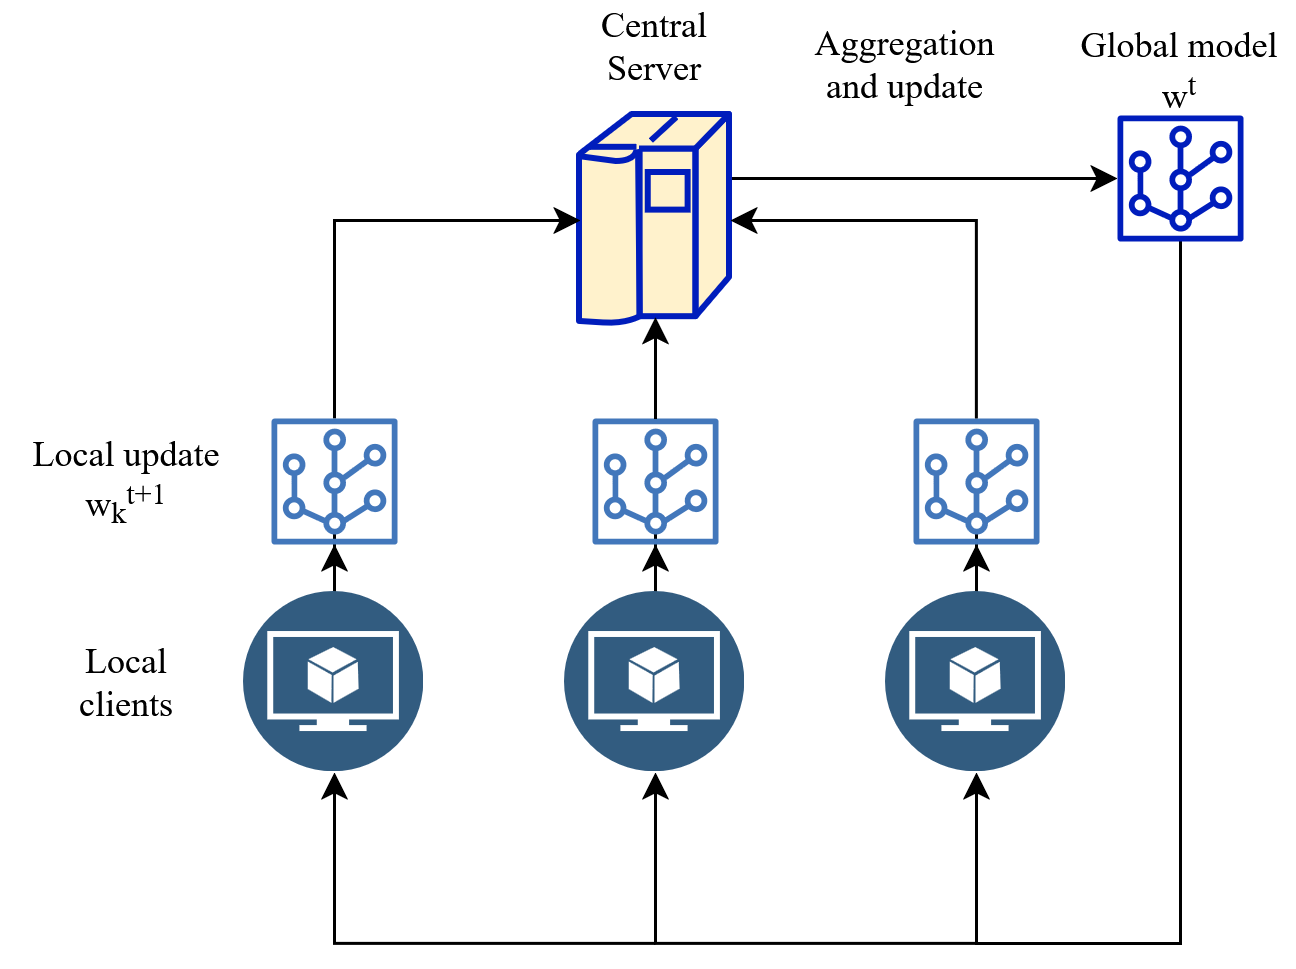
\includegraphics[scale=0.3]{federated_learning.png}
  \caption{Overview of the federated learning pipeline}
  \label{fig:fl-pipeline}
\end{figure}

In each communication round, the server distributes the current global model $w^t$ to a subset of clients. Each selected client initialises its local model with $w^t$ and performs $E$ epochs of stochastic gradient descent on its local data, producing updated parameters $w_k^{t+1}$. The server then aggregates these updates by computing a weighted average:
\begin{equation}
w^{t+1} = \sum_{k=1}^{K} \frac{n_k}{n} w_k^{t+1}
\end{equation}
By performing multiple local training epochs before communication, FedAvg significantly reduces communication costs compared to approaches that require gradient updates after every training step. 

Li et al. \cite{liFederatedLearningChallenges2020} surveyed the main challenges. 1) Communication costs are high when bandwidth is limited or models are large. 2) Participating devices vary in compute and connectivity. 3) Data across nodes is usually non-IID. 4) Shared updates can still leak information about training data.

\section{Handling Non-IID Data in Federated Learning}

Data distributions across participating nodes are rarely uniform. When each node holds data that is non-IID, local models trained on these subsets may diverge significantly from one another. Averaging such divergent models can produce a global model that performs poorly compared to one trained on centralised data.

FedAvg is particularly susceptible to this problem as it provides no way to limit how far local models can deviate from the global model during local training. Li et al. \cite{liFederatedOptimizationHeterogeneous2020} proposed FedProx to address this limitation. FedProx modifies the local objective function by adding a proximal term:
\begin{equation}
\min_{w} h_k(w; w^t) = F_k(w) + \frac{\mu}{2} | w - w^t |^2
\end{equation}
where $F_k(w)$ is the local loss, $w^t$ is the current global model and $\mu$ controls the strength of the penalty. This term penalises large deviations from the current global model. This modification provides convergence guarantees under heterogeneous data distributions, which FedAvg lacks. FedProx also accommodates systems heterogeneity by allowing nodes to perform variable amounts of local computation.

Other approaches have been proposed to tackle non-IID issues. Karimireddy et al. \cite{karimireddySCAFFOLDStochasticControlled2021} introduced SCAFFOLD, which uses control variates to correct for the drift in local updates. This reduces the variance caused by heterogeneous data. Wang et al. \cite{wangFederatedLearningMatched2020} proposed Federated Matched Averaging (FedMA), which aligns neurons across local models before averaging. This prevents neurons in different local models from learning equivalent features in different positions. Wang et al. \cite{wangTacklingObjectiveInconsistency2020} proposed FedNova, which normalises local updates to account for differences in the number of local training steps, correcting an inconsistency in FedAvg that is amplified under heterogeneous conditions. While this project focuses on FedAvg and FedProx, these alternative approaches provide context for understanding the breadth of strategies available for handling non-IID data in federated settings.

To evaluate federated learning methods under heterogeneous conditions, a consistent experimental method is required for simulating non-IID data splits. A widely adopted approach, introduced by Hsu et al. \cite{hsuMeasuringEffectsNonIdentical2019}, is to partition data across clients using a Dirichlet distribution over class labels, parameterised by a concentration parameter $\alpha$. Lower values of $\alpha$ produce more skewed label distributions across clients while higher values approach IID. This provides a controllable and reproducible way to study model behaviour across a wide range of heterogeneous conditions.
\section{Privacy in Federated Learning}
Federated learning avoids sharing raw data but this alone does not guarantee privacy. Kaissis et al. \cite{kaissisSecurePrivacypreservingFederated2020} noted that the model updates transmitted during training can be exploited to infer information about the underlying data. Model inversion attacks use model outputs or gradients to reconstruct approximations of training inputs \cite{fredriksonModelInversionAttacks2015}. Membership inference attacks determine whether a specific data point was in the training set by analysing the model's response to that input \cite{shokriMembershipInferenceAttacks2017}.

Several defence mechanisms have been proposed to strengthen privacy in federated learning. Bonawitz et al. \cite{bonawitzPracticalSecureAggregation2017} designed a practical secure aggregation protocol using pairwise masking to protect each participant's contribution. This enables the server to compute the sum of client updates without observing any individual update. This protocol is robust to client dropout, making it suitable for real-world deployments. Differential privacy provides a complementary approach by adding calibrated noise to the data or model updates to limit the information that can be inferred about any individual training example. Dwork et al. \cite{dworkCalibratingNoiseSensitivity2006} established the formal foundations of differential privacy, while Abadi et al. \cite{abadiDeepLearningDifferential2016} introduced DP-SGD, a training procedure that clips per-example gradients and adds noise during optimisation which enables deep learning models to be trained with formal privacy guarantees. These mechanisms can be combined with federated learning to provide stronger privacy protections, though they often introduce trade-offs with model accuracy.

\section{Federated Learning in Medical Imaging}
Federated learning has attracted significant interest in medical imaging, where data is inherently distributed across institutions and subject to strict privacy requirements. Rieke et al. \cite{riekeFutureDigitalHealth2020} outlined the potential of federated learning to enable collaborative model development across hospitals without centralising patient data, identifying it as a key enabler for the future of digital health. They noted that the heterogeneity of clinical data, arising from differences in imaging equipment, protocols, and patient demographics makes the non-IID problem particularly important in this domain.

Sheller et al. \cite{shellerFederatedLearningMedicine2020} demonstrated that federated learning could be applied to brain tumour segmentation across multiple institutions. They achieved performance comparable to centralised training while keeping patient data local. Their work provided early evidence that federated learning is viable in medical imaging tasks with complex, heterogeneous data. More recently, Dayan et al. \cite{dayanFederatedLearningPredicting2021} conducted one of the largest federated learning studies to date, training a model to predict clinical outcomes in COVID-19 patients across 20 institutions worldwide. Their model outperformed any single-institution model, which justifies federated learning in practice.

\section{Summary and Knowledge Gap}
The preceding sections have reviewed the relevant literature across skin disease classification, federated learning, non-IID data handling, privacy mechanisms, and federated learning in medical imaging. Several key gaps emerge from this review:

\begin{enumerate}
  \item \textbf{Limited evaluation of federated learning for multi-class skin disease classification.} Federated learning has been applied successfully in medical imaging, but primarily in radiology and pathology tasks with binary or few-class classification. Its performance on fine-grained, multi-class skin disease tasks with 20 or more classes has not been systematically studied.
  \item \textbf{Insufficient comparison of federated algorithms under realistic non-IID conditions.} While FedProx was designed to address the non-IID limitations of FedAvg, direct comparisons between the two on medical imaging tasks with realistic heterogeneity remain scarce. Most evaluations use standard benchmarks rather than domain-specific datasets where class imbalance and label skew occur.
  \item \textbf{Lack of practical guidance on federated learning trade-offs for clinical imaging.} Existing studies report accuracy but often do not systematically evaluate communication efficiency or per-class performance alongside non-IID sensitivity. Understanding these trade-offs is essential for informing whether federated learning is practical for real-world deployment.
\end{enumerate}

This project addresses these gaps by evaluating FedAvg and FedProx on a 30-class skin disease dataset to simulate realistic data heterogeneity. By comparing these approaches against a centralised baseline on classification accuracy, communication efficiency, and behaviour under non-IID distributions, this project aims to provide practical insight into the suitability of federated learning for fine-grained medical image classification.


\chapter{Methodology}

\section{Project Aims}
Based on the knowledge gaps identified in the preceding chapter, this project has the following aims:
\begin{itemize}
  \item Train a centralised ResNet classifier on 20,000 images across 30 classes to establish an upper-bound benchmark
  \item Run FedAvg and FedProx on the same data, partitioned into IID and Dirichlet non-IID splits across simulated clients
  \item Report how each federated method degrades from the centralised baseline as heterogeneity increases, and what it costs in communication rounds
\end{itemize}

\section{Experimental Pipeline}
This project follows a three-stage experimental pipeline: centralised baseline training, federated learning implementation, and comparative evaluation. All experiments will be implemented in Python using PyTorch.

\subsection{Dataset}
Two publicly available skin disease image datasets from Kaggle will be used. The first, the Skin Diseases and Cancer Comprehensive Dataset, contains approximately 13,000 images across 24 diagnostic classes \cite{SkinDiseasesCancer}. The second, a larger balanced skin disease dataset, contains approximately 262,000 images across 34 classes \cite{MassiveSkinDisease}. Table~\ref{tab:datasets} summarises the two datasets. The final dataset composition will be determined during implementation; options include using either dataset independently, merging them with a unified class mapping, or using a subsampled combination to manage compute requirements. Images will be resized to a uniform resolution and normalised to standardise input across all experiments. Standard data augmentation techniques such as random horizontal flipping, rotation, and colour jittering will be applied during training to improve generalisation. The dataset will be split into training, validation, and test sets, with the test set held centrally and kept consistent across all experiments to ensure fair comparison. 

\begin{table}[H]
  \centering
  \caption{Summary statistics of the datasets used in this project.}
  \label{tab:datasets}
  \renewcommand{\arraystretch}{1.3}
  \begin{tabular}{|l|c|c|}
    \hline
    \textbf{Property} & \textbf{Dataset 1} & \textbf{Dataset 2} \\ \hline
    Name & Skin Diseases + Cancer & Massive Skin Disease \\ \hline
    Source & Kaggle & Kaggle \\ \hline
    Total images & $\sim$13,000 & $\sim$262,000 \\ \hline
    Number of classes & 24 & 34 \\ \hline
    Image type & Clinical photographs & Clinical photographs \\ \hline
    Class balance & Imbalanced & Balanced \\ \hline
  \end{tabular}
\end{table}

\subsection{Centralised Baseline}
A ResNet-18 architecture pre-trained on ImageNet will be used as the primary classification model across all experiments, selected for its established performance in image classification tasks \cite{heDeepResidualLearning2015}. If compute resources permit, ResNet-50 will also be evaluated to assess the impact of model capacity on classification performance. The baseline will be trained on the full training set in a standard centralised setting, with all data aggregated on a single machine. This represents an upper bound on classification performance. Training will use stochastic gradient descent with momentum, with learning rate, batch size, and number of epochs tuned on the validation set. To account for variability, experiments will be repeated across multiple random seeds and results reported as mean and standard deviation.
\subsection{Federated Learning}
The training set will be partitioned across $K$ simulated client nodes to replicate a distributed healthcare environment. Two partitioning strategies will be used. In the IID setting, data will be distributed uniformly at random across clients, ensuring each client holds a roughly representative subset. In the non-IID setting, a Dirichlet distribution with concentration parameter $\alpha$ will be used to create heterogeneous label distributions across clients, where lower values of $\alpha$ produce greater skew \cite{hsuMeasuringEffectsNonIdentical2019}. Multiple values of $\alpha$ (for example, $\alpha\in\{0.1,0.5,1.0\}$) will be tested to evaluate model behaviour under varying degrees of heterogeneity. The inherent class imbalance in the dataset will be considered when designing the partitioning, as it interacts with the label skew introduced by non-IID splits.

FedAvg and FedProx will each be implemented following the procedures described in Chapter 2. The same ResNet-18 architecture and preprocessing pipeline used in the centralised baseline will be applied to ensure that differences in performance are attributable to the training method rather than the model. 

In each communication round, a fraction $C = 0.5$ of $K = 10$ clients will be selected to participate. Each selected client will train on its local data for $E = 5$ local epochs with batch size $B = 32$, then send its updated model parameters to the central server for aggregation. 

For FedProx, the proximal term weight $\mu$ will be tuned over $\mu \in \{0.001, 0.01, 0.1, 1.0\}$ using the validation set. This allows assessment of its impact under different levels of regularisation.

Training will run for up to $T = 100$ communication rounds. Early stopping will be applied based on validation performance.

\subsection{Evaluation}

All approaches will be evaluated on the same held-out test set using the following metrics.

\begin{itemize}
  \item \textbf{Classification accuracy}: overall accuracy on the test set.
  \item \textbf{Per-class performance}: precision, recall, and F1-score per class to assess behaviour on minority classes, which is particularly important given dataset imbalance.
  \item \textbf{Communication efficiency}: the number of communication rounds required to reach a target accuracy and the total volume of parameter data transmitted between clients and server.
  \item \textbf{Non-IID sensitivity}: accuracy as a function of the Dirichlet concentration parameter $\alpha$, measuring how each method degrades under increasing data heterogeneity.
\end{itemize}
Results from FedAvg and FedProx will be compared against each other and against the centralised baseline across all metrics. All experiments will be repeated over multiple random seeds to ensure reported differences are statistically meaningful.

\section{Ethical Considerations}
This project uses only publicly available skin disease image datasets obtained from Kaggle. Both datasets have been released by their authors for research and educational purposes, and contain no directly identifying patient information such as names or dates of birth. No new patient data will be collected, and no human or animal subjects will be involved in the research. For these reasons, formal ethics approval is not required for this project.

Several ethical considerations remain relevant. Publicly released medical image datasets may still carry risks of re-identification. This project will treat all data as sensitive and will not attempt to link images back to individuals or external sources.

Skin disease classifiers are known to exhibit performance disparities across skin tones, as publicly available datasets are often skewed toward lighter skin types. Any results produced by this project will be interpreted with this limitation in mind and per-class performance metrics will be reported to surface any systematic disparities that arise.

While this project is a simulation and does not involve real clinical deployment, the broader motivation carries downstream implications for patient privacy, model accountability, and the trustworthiness of clinical AI systems. This project is a methodological evaluation and no diagnostic claims follow from it.

All code, experimental configurations, and results will be managed with version control to support reproducibility, and the datasets used will be properly cited so that others can verify and build upon the work.



\chapter{Study 1: Centralised Baseline and IID Federated Learning}

\section{Aims}
\begin{itemize}
  \item Establish centralised ResNet-18 baseline performance on the 30-class dataset.
  \item Evaluate FedAvg and FedProx under IID partitioning to verify that federated training approaches the centralised upper bound when data is homogeneous.
\end{itemize}

\section{Methods}
\begin{itemize}
  \item Centralised training as described in Chapter 3, with hyperparameters tuned on the validation set.
  \item FedAvg and FedProx with $K = 10$ clients, $C = 0.5$, $E = 5$, $B = 32$, uniform random data partitioning.
\end{itemize}

\section{Results}
\begin{itemize}
  \item To be completed: accuracy and per-class metrics for the centralised baseline.
  \item To be completed: federated accuracy versus communication rounds under IID conditions.
\end{itemize}

\section{Discussion}
\begin{itemize}
  \item To be completed: gap between federated and centralised performance under IID conditions.
\end{itemize}

\chapter{Study 2: Federated Learning under Non-IID Conditions}

\section{Aims}
\begin{itemize}
  \item Evaluate how FedAvg and FedProx degrade as data heterogeneity increases.
  \item Assess whether the FedProx proximal term improves stability and accuracy under label skew.
\end{itemize}

\section{Methods}
\begin{itemize}
  \item Dirichlet partitioning with $\alpha \in \{0.1, 0.5, 1.0\}$.
  \item FedProx proximal weight tuned over $\mu \in \{0.001, 0.01, 0.1, 1.0\}$.
\end{itemize}

\section{Results}
\begin{itemize}
  \item To be completed: accuracy as a function of $\alpha$ for both methods.
  \item To be completed: communication rounds to target accuracy, per-class performance on minority classes.
\end{itemize}

\section{Discussion}
\begin{itemize}
  \item To be completed: comparison of FedAvg and FedProx degradation, practical implications for federated medical imaging.
\end{itemize}

\chapter{General Discussion and Conclusions}
\section{Summary}
\begin{itemize}
  \item To be completed: summary of baseline, IID, and non-IID findings.
\end{itemize}
\section{Discussion and Future Work}
\begin{itemize}
  \item To be completed: how the two studies together answer the project aims.
  \item Planned future directions: stronger architectures such as Vision Transformers, non-IID improvements, communication optimisations.
\end{itemize}
\section{Conclusions}
\begin{itemize}
  \item To be completed: overall assessment of whether federated learning is a viable substitute for centralised training in this setting, and under what heterogeneity conditions.
\end{itemize}

\cleardoublepage

\addcontentsline{toc}{chapter}{Bibliography}
\bibliographystyle{unsrtnat}
\bibliography{references}

\appendix

% Chapters after the \appendix command are lettered, not numbered.
% Setting apart the appendices in the table of contents is awkward:

\newpage
\addcontentsline{toc}{part}{Appendices}
\mbox{}
\newpage

% The \mbox{} command between two \newpage commands gives a blank page.
% In the contents, the ``Appendices'' heading is shown as being on this
% blank page, which is the page before the first appendix.  This stops the
% first appendix from be listed ABOVE the word ``Appendices'' in the
% table of contents.

% \include appendix chapters here.

\chapter{Program listings}
Code and experimental configurations will be made available via a GitHub repository, with directions provided in the final thesis.

\end{document}